\clearpage
\section{Interpretation}\label{sec:Interpretation}
Eine Messung unterscheidet sich durch die unterschiedlichen Messparameter, sowie durch den Messaufbau (Wohnung / Labor / Haus). Um einen Vergleich ziehen zu können, wird daher nach diesen beiden Hauptmerkmalen unterschieden.

Dieser Vergleich bezieht sich auf die selbe Testumgebung, jedoch mit unterschiedlichen Messreihen. Im Anschluss soll gezeigt werden wie sich die einzelnen Mesh-Netzwerke bei veränderten Messreihen verändern.

Durch die in Abbildung \ref{fig:Latenzzeiten_per_Hop_Messreihen} dargestellten Latenzzeiten wird ersichtlich das Bluetooth-Mesh am anfälligsten auf die Erhöhung der Payload reagiert. Eine detaillierte Analyse zu diesem Phänomen wird in Abschnitt \ref{subsubsec:FazitBluetoothMesh} durchgeführt. Die Verzögerung bleibt bei Zigbee und Thread trotz Erhöhung der Paketlänge stabil.

\begin{figure}[H]
	\centering
	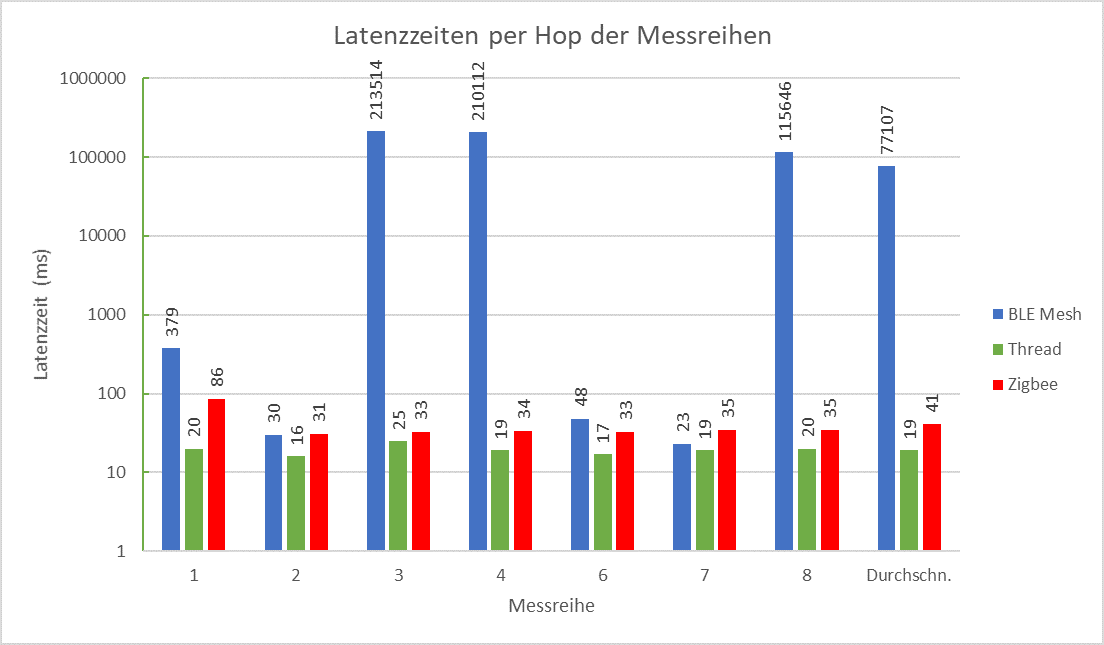
\includegraphics[width=1.0\textwidth]{Latenzzeiten_per_Hop_Messreihen.png}
	\caption{Durchschnittliche Latenzzeit per Hop der einzelnen Messreihen im Vergleich}\label{fig:Latenzzeiten_per_Hop_Messreihen}
\end{figure}

Ein Änderung des Traffic Generation Mode von Random auf Sequentiell bewirkt bei Bluetooth-Mesh eine drastische Abnahme der Latenz. Bei Zigbee ist zwischen der Messreihe 1 und 2 ebenfalls eine Abnahme zu verzeichnen, welche jedoch nicht zwischen der Reihe 3 und 4 feststellbar ist. Somit muss ein anderer Einfluss für die Abnahme verantwortlich sein (in Abschnitt \ref{subsubsec:FazitZigbee} untersucht). Die Änderung des Traffic Generation Mode wirkt bei Thread ebenfalls zu einer Verbesserung der Latenz.

Das Senken der Message Dichte führt bei Bluetooth-Mesh zu einer markanten Abnahme der Latenz. Bei Thread und Zigbee bleibt die Latenz nahezu identisch.

Die Einbringung von Störungen hat lediglich bei Bluetooth-Mesh einen negativen Einfluss, wodurch sich die Latenzzeit erhöht. 


\subsection{Vergleich Testumgebungen}\label{subsec:VergleichTestumgebungen}
Dieser Vergleich bezieht sich auf die selbe Messreihe, jedoch in unterschiedlichen Testumgebungen. Als Referenz wurde die Messreihe 2 ausgewählt, da diese für alle Testumgebung repräsentative Resultate enthält. Im Anschluss soll gezeigt werden wie sich die einzelnen Mesh-Netzwerke bei veränderten Testumgebungen verändern.

\subsubsection{Latenzzeit}\label{subsec:VergleichLatenzzeitTestumgebungen}
\begin{figure}[H]
	\centering
	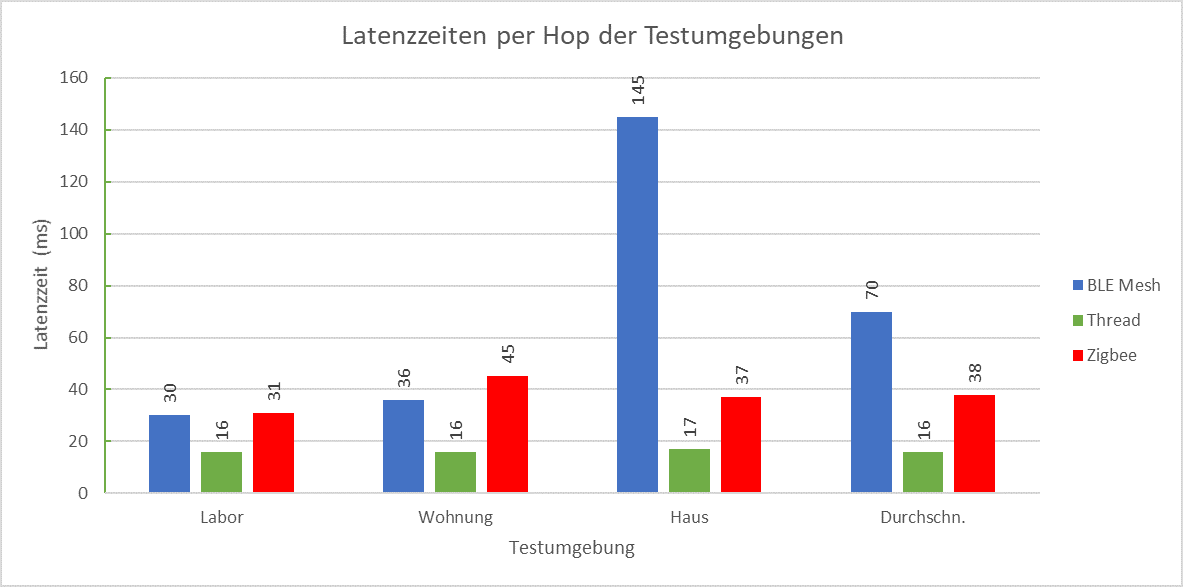
\includegraphics[width=1.0\textwidth]{Latenzzeiten_per_Hop_Testumgebungen.png}
	\caption{Durchschnittliche Latenzzeit per Hop der einzelnen Testumgebungen im Vergleich}\label{fig:Latenzzeiten_per_Hop_Testumgebungen}
\end{figure}

Die Abbildung \ref{fig:Latenzzeiten_per_Hop_Testumgebungen} zeigt das die Testumgebung Labor für alle Netzwerke die geringste Verzögerung aufweist. Bluetooth-Mesh erfährt bei weiter Streuung der Teilnehmer, wie sie im Haus anzutreffen ist, die grösste Steigerung der Latenz. Zigbee erhält in der Wohnung eine kaum relevante Erhöhung der Verzögerung. Thread zeichnet sich als unabhängig bezüglich der Testumgebung aus. 

\subsubsection{Durchsatz}\label{subsec:VergleichDurchsatzTestumgebungen}
\begin{figure}[H]
	\centering
	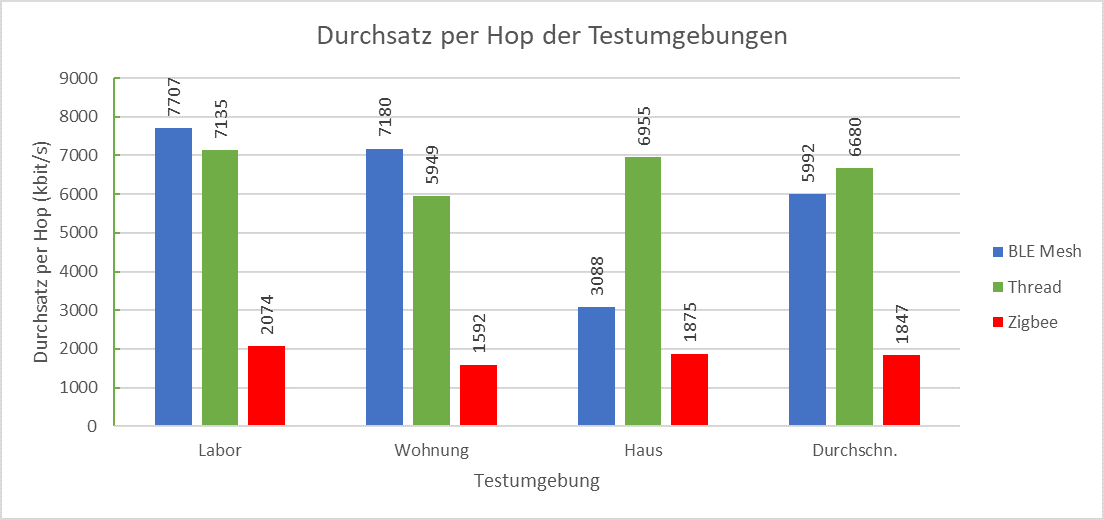
\includegraphics[width=1.0\textwidth]{Durchsatz_per_Hop_Testumgebungen.png}
	\caption{Durchschnittlicher Durchsatz per Hop der einzelnen Testumgebungen im Vergleich}\label{fig:Durchsätze_per_Hop_Testumgebungen}
\end{figure}

Ähnlich zu den Betrachtungen der Latenzzeit, zeigt die Abbildung \ref{fig:Durchsätze_per_Hop_Testumgebungen} den höchsten Durchsatz im Testaufbau Labor. Bluetooth-Mesh erfährt den grössten Einfluss durch ein ändern der Topologie. 

\subsubsection{Paketverlust}\label{subsec:VergleichPaketverlustTestumgebungen}
\begin{figure}[H]
	\centering
	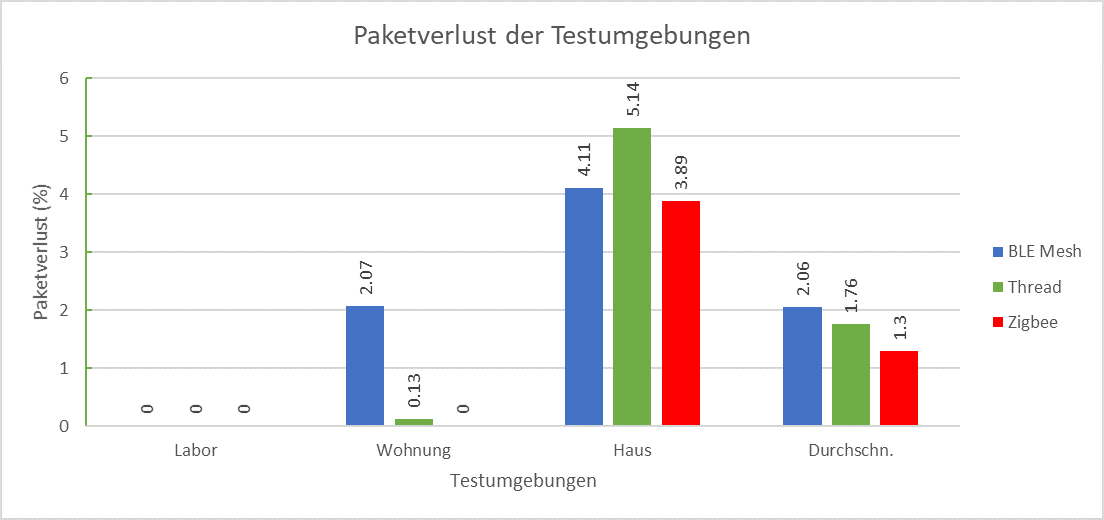
\includegraphics[width=1.0\textwidth]{Paketverlust_Testumgebungen.png}
	\caption{Durchschnittlicher Paketverlust der einzelnen Testumgebungen im Vergleich}\label{fig:PaketverlusteTestumgebungen}
\end{figure}

Abbildung \ref{fig:Durchsätze_per_Hop_Testumgebungen} zeigt das im Labor-Aufbau alle Netzwerke vollkommen zuverlässig arbeiten. In der Wohnung erlebt Bluetooth-Mesh einen geringen Anstieg des Paketverlusts. Bei Thread ist die Änderung kaum relevant. Alle Netzwerke erfahren bei starker Verzweigung des Netzwerks einen Anstieg der Verlustrate wie es bei der Haus-Topologie zu sehen ist. 

\subsection{Fazit}\label{subsec:FazitVergleich}
Alle Mesh-Netzwerke mussten diversen Tests standhalten. Die Ergebnisse aus den Messreihen 1 bis 4 aus allen Testumgebungen wurden als Durchschnittswert zusammengefasst, um einen finalen Vergleich zu erzielen. Die Abbildung \ref{fig:Messresultate_Fazit} zeigt alle Ergebnisse auf einen Blick. Schlussendlich lässt sich Thread als klarer Sieger erkennen. Dieser Network-Stack hat die Tests am besten absolviert. Auf dem zweiten Platz steht Zigbee, welches mit seiner konstanten Latenz und als zuverlässigstes Protokoll die Daten verarbeiten konnte. Dabei gilt zu beachten das bei Zigbee die Hops nicht berücksichtigt wurden. Bluetooth-Mesh kann durch den niedrigen Energiebedarf brillieren, schneidet jedoch in Sachen Performance deutlich schlechter als seine Konkurrenten ab. Im Anschluss wird jedes Protokoll genauer analysiert und auf die Vor- und Nachteile, sowie mögliche Verbesserungen eingegangen. 

\begin{figure}[H]
	\centering
	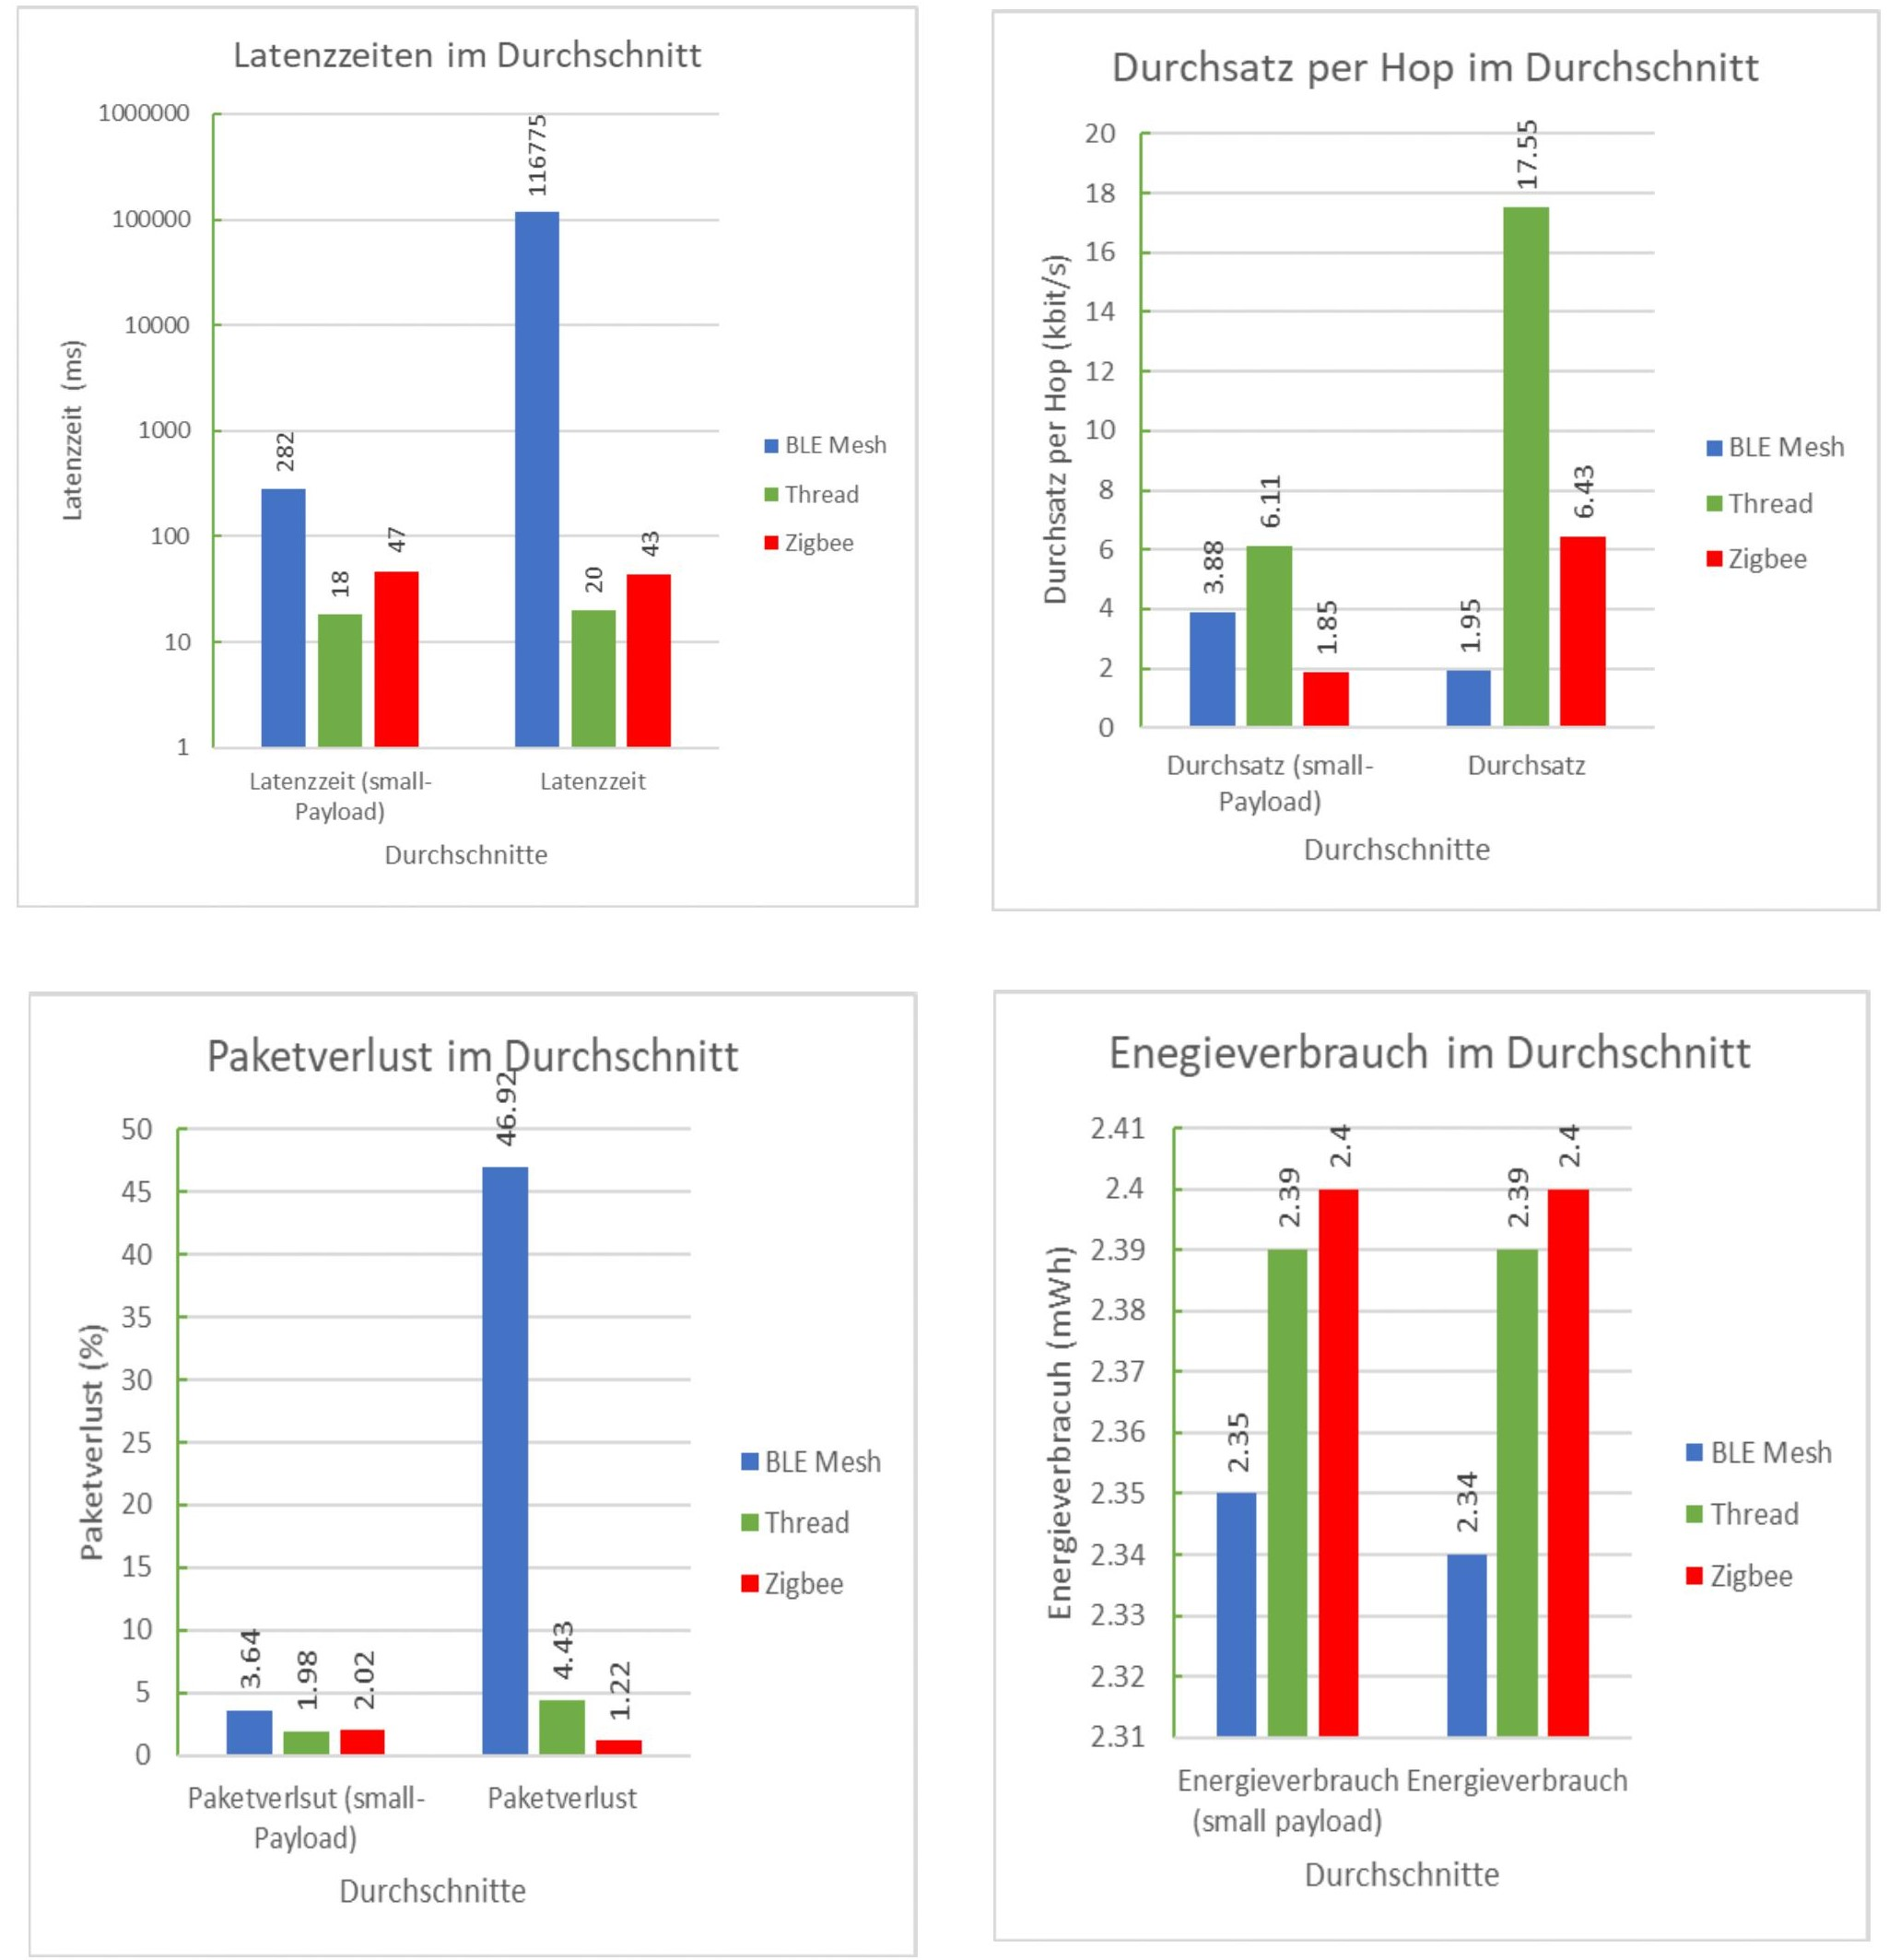
\includegraphics[width=0.95\textwidth]{Messresultate_Fazit.jpg}
	\caption{Durchschnittliche Messgrössen im Vergleich inkl. separater Betrachtung der Messergebnisse, welche mit 8-Byte Paketlänge erzielt wurden}\label{fig:Messresultate_Fazit}
\end{figure}

\newpage
\subsubsection{Thread}\label{subsubsec:FazitThread}
Wie aus den vorhergehenden Kapiteln ersichtlich hat der Thread Stack die Messungen am besten abgeschlossen. Das bedeutet aber nicht unbedingt, dass der Stack der Beste ist. Es ist klar zu erkennen, dass der Thread Stack dank seiner automatischen Ernennung von Routing-Knoten, sich seiner Umgebung gut anpassen kann. Die Latenzzeit der gesendeten Nachrichten ändert sich in verschiedenen Umgebungen nur minimal. Das bedeutet, dass sich der Stack sehr gut für eine Hausautomation eignet. Wenn sich Sensoren oder Aktoren verschieben, z.B. wenn eine Lampe einen neuen Standort erhaltet, erkennt dies der Stack und kann das Routing der Knoten anpassen. Da sich das Netz sehr gut erweitern lässt und sich die Latenzzeiten eher tief zeigen, kann das Mesh-Netzwerk ausserdem gut für Industrieanwendungen verwendet werden. 

Durch das automatische Routen der Knoten, entsteht auf den einzelnen Nodes jedoch ein Overhead, der zum Beispiel BT-Mesh nicht hat. Aus diesem Grund ist der Energieverbrauch auf den Knoten höher, was sich auch in der Abbildung \ref{fig:EnergieverbrauchMessreihen} zeigt. Dies ist keine repräsentative Messung, da nur die aktiven Radio Zeiten gemessen wurden, es könnte trotzdem die vorherige These mit dem Overhead bestätigen. 

Anders als bei BT-Mesh können mit dem IEEE 802.15.4 und dem 6LoWPAN Layer grössere Pakete versendet werden. Das bedeutet, dass die Segmentierung im Gegensatz zu BT Mesh später stattfindet. Dies erklärt das Phänomen, dass sich der Durchsatz mit steigender Payload vergrössert. Der Thread Stack erreicht bei manchen Messreihen einen Durchsatz von bis zu 32 kbit pro Sekunde. Dies ist jedoch eher unwahrscheinlich. Da bei den Durchschnittsberechnungen kein Median verwendet wurde, können Extremwerte den Durchschnitt verfälschen. Es gab sehr wenige Latenzmessungen, die fehlerhaft waren und eine Latenz unter 0.5ms aufwiesen. Durch diesen Fehler wurde der Durchsatz in der Auswertung unwahrscheinlich hoch. 

\subsubsection{Zigbee}\label{subsubsec:FazitZigbee}
Die Resultate und Vergleiche aus den vorhergehenden Abschnitten zeigen, dass das Zigbee Protokoll in dieser Implementation eine solide Performance abliefert.
Auch wenn Zigbee nicht ganz an jene Leistung von Thread herankommt, bestätigen die Ergebnisse wieso es zurzeit das am weitesten verbreiteten WPAN Protokoll ist.

Die durchschnittlichen Latenzzeiten liegen zwischen 30 und 50 Millisekunden. Damit schneidet Zigbee besser ab als Bluetooth jedoch liegt es hinter jenen Durchschnittswerten von Thread.
Dies kommt nicht allzu überraschend.
Sehr interessant zu beobachten sind die Verteilungen der Latenzzeiten, wie sie beispielsweise in Abbildung \ref{fig:VerteilungderLatenzzeiten} zu sehen sind.
Anders als beispielsweise Thread weist Zigbee dort deutliche Peaks bei 40ms und 70ms auf.
Diese Beobachtung kann bei sämtlichen Messresultaten gemacht werden.
Ausreisser nach unten gibt es praktisch keine und solche nach oben nur sehr vereinzelt.
Es kann also festgestellt werden, dass bei Zigbee mit einer minimalen Latenzzeit von ca. 30ms gerechnet werden muss, diese aber in den seltensten Fällen deutlich überschreitet.
Zigbee wäre also auch für eher zeitkritische Anwendungen geeignet da die Latenzzeiten deterministisch sind.
In diesen Zusammenhang nochmals zu erwähnen ist, das Fehlen der Information über die Anzahl Hops die ein Paket während dem Benchmark genommen hat.
Es kann davon ausgegangen werden, dass der zweite Peak bei 70ms Latenzzeit diesem Problem verschuldet ist.
Wenn also die Anzahl Hops erfasst werden könnte, dürfte sich die Verteilung der Latenzzeiten wohl nochmals reduzieren.

Die Ergebnisse aus Abbildung \ref{fig:Latenzzeiten_per_Hop_Messreihen} zeigen eine weitere interessante Eigenschaft von Zigbee.
In Messreihe 1 beträgt die durchschnittliche Latenzzeit mit 86ms mehr als das doppelte als in den übrigen Messreihen.
Die Ursache dafür kann nicht abschliessend geklärt werden.
Jedoch liegt die Vermutung nahe, dass sich das Mesh Netz während dieser Messreihe noch nicht komplett aufgebaut respektive das \textit{Commissioning} und \textit{Route Discovery} noch nicht abgeschlossen war.
Dies verursachte zusätzlichen Traffic und beeinflusste den Benchmark.

Auffallend tief ist auch der Paketverlust.
In den meisten Fällen lag dieser sogar bei 0 Prozent.
Hier macht sich das CSMA\slash CA des IEEE 802.15.4 MAC Layers bemerkbar.
Zudem wirkt sich hier wohl die Unicast Adressierung innerhalb von Zigbee positiv aus.
Die Gesamtbelastung des Netzes kann dadurch deutlich minimiert werden.

Die Erhöhung der Payload von 8 auf 50 Byte hat die Latenzzeiten bei den Zigbee Messungen nicht merklich beeinflusst.
Somit steigt auch der Durchsatz mit grösserer Payload.
Da die Segmentierung dank IEEE 802.15.4 erst ab 127 Byte Framelänge startet ist dies auch nicht weiter verwunderlich.
Gegenüber BT Mesh haben Zigbee wie auch Thread den klaren Vorteil grössere Payloads versenden zu können ohne segmentieren zu müssen.

Zigbee brilliert in den Anwendungen in denen es sowieso bereits verbreitet eingesetzt wird.
Sei dies eine komplette Hausautomation oder eine Lichtsteuerung, bis zu einer Netzwerkgrösse von ungefähr 200 Nodes mit einigermassen kleinem Verkehrsaufkommen ist Zigbee die ideale Wahl.
Ergänzt durch die \textit{Zigbee Cluster Library} welche die Systeme herstellerunabhängig macht wird Zigbee noch interessanter.


\subsubsection{Bluetooth Mesh}\label{subsubsec:FazitBluetoothMesh}
Die Performance von Bluetooth-Mesh ist stark von der Belastung abhängig, wie aus dem Abschnitt \ref{subsec:Interpretation} zu erkennen ist. Der grösste Einfluss auf die Performance hatte die Länge der gesendeten Nachrichten. Dies hat seinen Ursprung das ein einzelnes Bluetooth-Mesh-Paket lediglich 10-Byte aufnehmen kann. Der Stack beginnt mit der Segmentierung der Daten in mehrere kleine Pakete. Bei 32-Byte sind dies bereits 4 Frames. Damit ist der komplette Network-Stack überfordert. 

\begin{figure}[H]
	\centering
	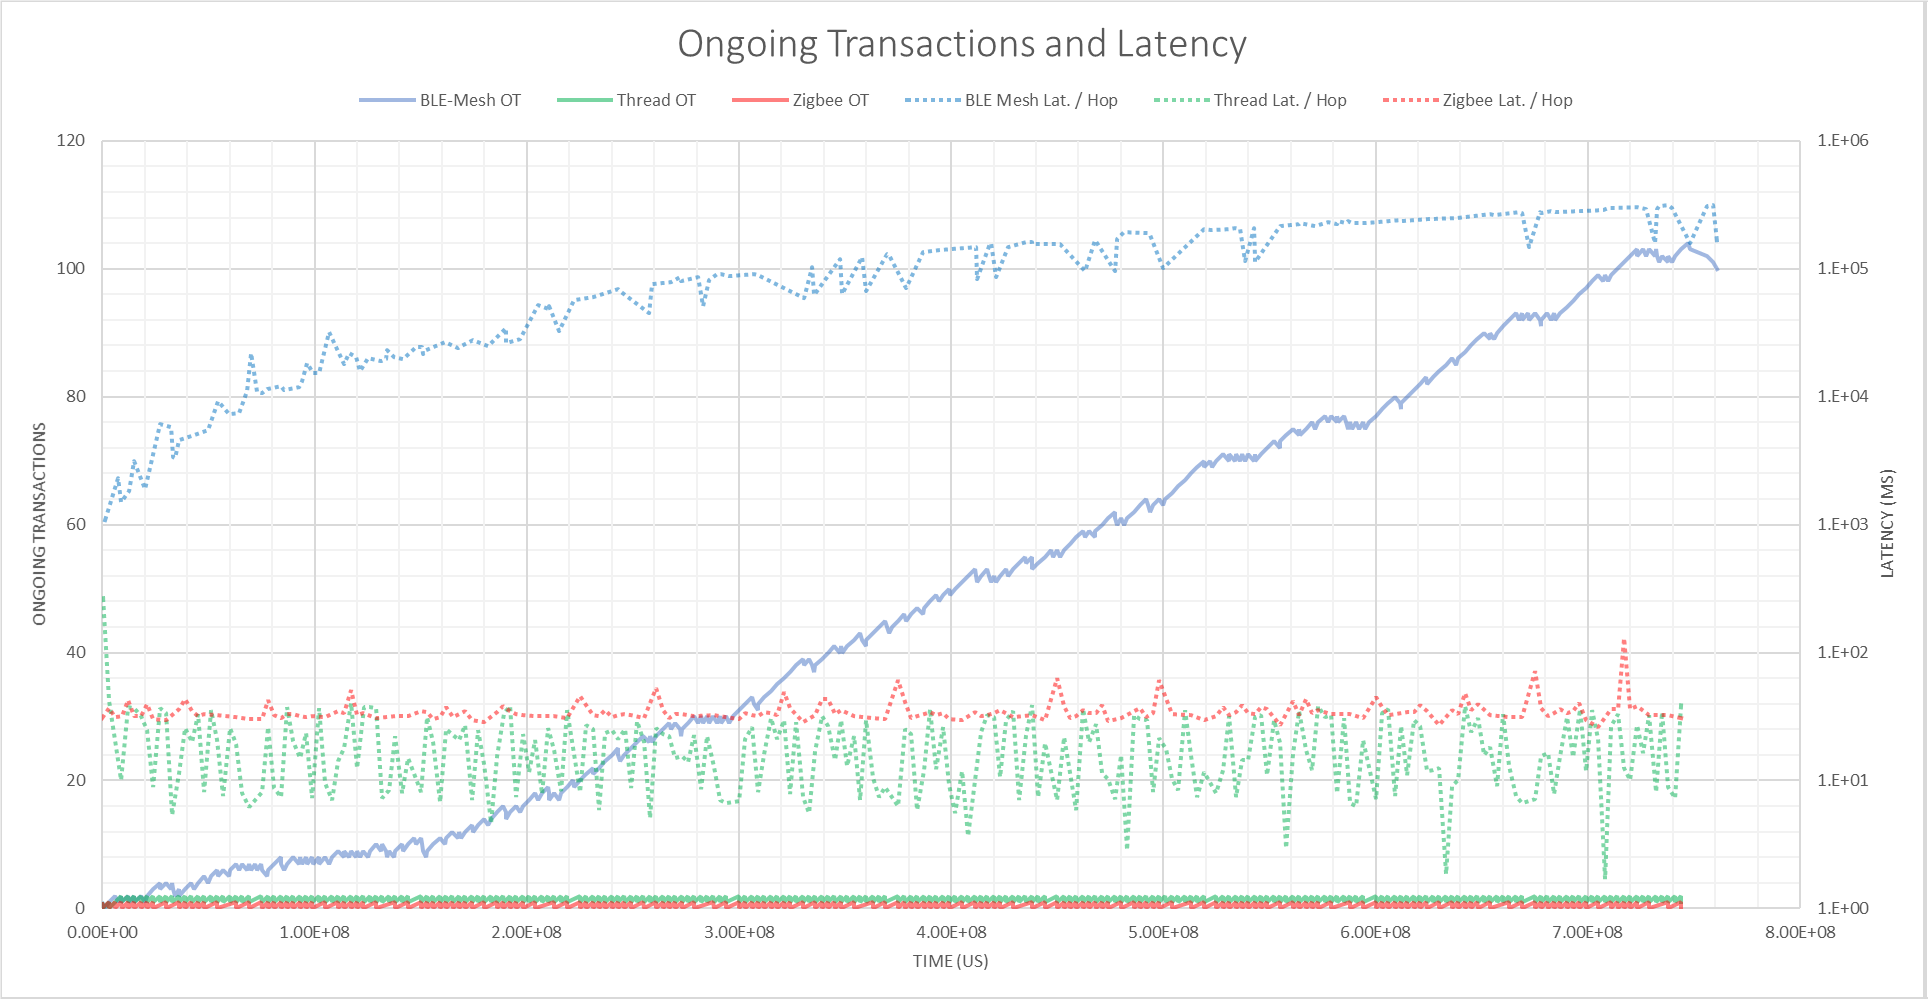
\includegraphics[width=1.0\textwidth]{Bluetooth_Mesh_Big_Payload_Issue.png}
	\caption{Ongoing Transactions und Latenzzeiten einer Messung mit 32Byte Paketlänge}\label{fig:Bluetooth_Mesh_Big_Payload_Issue}
\end{figure}

Abbildung \ref{fig:Bluetooth_Mesh_Big_Payload_Issue} zeigt eine Messung mit 32-Byte Payload, einer Message-Dichte von 3 Sekunden / Message welche Sequenziell versendet wurden. Dabei ist zu erkennen, dass die Anzahl der Ongoing Transactions immer weiter ansteigt. Lediglich in der Nachtbearbeitungszeit sinkt die Kurve wieder. Dies deutet darauf hin das zu viel Traffic im Netz gesendet wird. Angelehnt an die Ongoing Transactions steigt die Latenz von einer Sekunde auf einige 100 Sekunden an.

Vermutlich entsteht eine zu hohe Message-Dichte, da zu viele Relay-Nodes jede empfangene Message wiederholen. Durch deaktivieren einiger Relays könnte der Netzaufbau entlastet werden. Jedoch erfordern solche manuellen Eingriffe Fachwissen und verringern die Ausfallsicherheit des Netzes. 
